\section*{Algebra}
\subsection*{Throwing Dice (CSES 1092)}
\textbf{Hint1}
\\\\
Llamemos $f(n)$ son las formas de obtener suma $n$ lanzando el dado. Notemos que $f(n-1)$ son las formas de obtener $f(n)$ si el último dado sale $1$.
\\\\
\textbf{Hint2}
\\\\
¿La observación de $f(n-1)$ también se cumple para $f(n-2)$? ¿Qué hay de $f(n-3)$?
\\\\
\textbf{Solución}
\\\\
A primer vistazo, este problema parece de combinatoria o DP, pero en realidad este problema se resuelve usando recurrencias. El último dado tiene $6$ resultados diferentes, si el último dado muestra $1$, la suma de los lanzamientos anteriores debe ser $n-1$ o de lo contrario nuestra suma final no podría ser $n$. Esto se cumple para todos los resultados del dado, es decir, que si nos sale $6$, la suma acumulada debería ser $n-6$. Esta observación nos sugiere que
\[f(n)=f(n-1)+f(n-2)+f(n-3)+f(n-4)+f(n-5)+f(n-6)\]
Como $n\leq10^{18}$ no podemos calcular $f(n)$ iterativametne. Aplicando exponenciación de matrices, la matriz de transición es:
\[
\begin{pmatrix} f(n)\\ f(n-1)\\ f(n-2)\\ f(n-3)\\ f(n-4)\\ f(n-5) \end{pmatrix}
=
\begin{pmatrix}
1 & 1 & 1 & 1 & 1 & 1 \\
1 & 0 & 0 & 0 & 0 & 0 \\
0 & 1 & 0 & 0 & 0 & 0 \\
0 & 0 & 1 & 0 & 0 & 0 \\
0 & 0 & 0 & 1 & 0 & 0 \\
0 & 0 & 0 & 0 & 1 & 0
\end{pmatrix}
\begin{pmatrix} f(n-1)\\ f(n-2)\\ f(n-3)\\ f(n-4)\\ f(n-5)\\ f(n-6) \end{pmatrix}
\]
Sólo hay $1$ forma de obtener $1$ como suma (y $0$ formas para números negativos), entonces podemos simplemente calcular:
\[
\begin{pmatrix} f(n)\\ \vdots\\ f(n-5) \end{pmatrix}
=
\begin{pmatrix}
1 & 1 & 1 & 1 & 1 & 1 \\
1 & 0 & 0 & 0 & 0 & 0 \\
0 & 1 & 0 & 0 & 0 & 0 \\
0 & 0 & 1 & 0 & 0 & 0 \\
0 & 0 & 0 & 1 & 0 & 0 \\
0 & 0 & 0 & 0 & 1 & 0
\end{pmatrix}^{n}
\begin{pmatrix} 1\\ 0\\ 0\\ 0\\ 0\\ 0 \end{pmatrix}
\]
La complejidad es $O(6^3 \log n) = O(\log n)$.
\\\\
\textbf{Código}
\\\\
Ver \href{https://cses.fi/paste/48e6570bd3a36951107242d/}{código}.

\subsection*{Cowmpany Compensation (Codeforces 995F)}
\textbf{Hint1}
\\\\
Considera una función $f(v,x)$, el número de formas de asignar salarios al subárbol $v$ asignando salario $x$ a $v$. ¿De qué depende el valor de $f(v,x)$?
\\\\Notemos que si $v$ es una hoja, $f(v,x)=1$.
\\\\
\textbf{Hint2}
\\\\
 Si $v$ es un vértice cuyos únicos $k$ hijos son hojas, $f(v,x)=\prod_{1}^{k} \sum_{i}^{x} f(s_k,i)$, donde $s_k$ es el $k$-ésimo hijo de $v$
\\\\
\textbf{Hint3}
\\\\
Podemos calcular $f(v,x)$ para $x \in \{1,2,...,n+1\}$ con $n\leq 3000$ en tiempo. Sin embargo, $d\leq 10^9$, como evaluamos polinomios para valores muy grandes en $O(n)$?
\\\\
\textbf{Solución}
\\\\
Definimos $f(v,x)$ como el número de formas de asignar salarios al
subárbol de $v$ dado que $v$ tiene salario $x$:
\[
f(v,x)=\prod_{i=1}^{k} \sum_{j=1}^{x} f(s_i,j)
\]
donde $s_1,\ldots,s_k$ son los hijos de $v$. Para cualquier nodo $v$,
definimos $g(v,x)$ como las formas de asignar salario \textbf{a lo
más} $x$ al subárbol de $v$:
\[
g(v,x)=\sum_{j=1}^{x} f(v,j)
\]
Notemos que la respuesta final es $g(1,d)$.
\\\\
\textbf{¿Qué grado tiene este polinomio?} Si $v$ es una hoja,
$f(v,x)=1$ (grado 0) y $g(v,x)=x$ (grado 1). En general:
\[
f(v,x)=\prod_{i=1}^{k}g(s_i,x)
\]
los grados de los $g(s_i,x)$ se suman, entonces:
\[
\deg(f(v,x))=\sum_{i=1}^{k} \deg(g(s_i,x))
\]
Y como $g(v,x)=\sum_{j=1}^{x}f(v,j)$ sube el grado en 1, el grado
de $g(v,x)$ es igual al \textbf{número de nodos en el subárbol de $v$}.
Por lo tanto $\deg(g(1,x)) = n$ el número total de vértices.
\\\\
Podemos calcular $g(1,1), g(1,2), \ldots, g(1,n+1)$ en $O(n^2)$ con DP procesando los nodos de hojas a raíz. Para cada nodo $v$ y cada $x$, calculamos $f(v,x) = \prod_{i=1}^{k} g(s_i,x)$ y luego $g(v,x) = g(v,x-1) + f(v,x)$, guardando ambos valores en memoria
para evitar repetir cálculos. Con $n+1$ puntos evaluados en $x=1,2,\ldots,n+1$ (puntos consecutivos), aplicamos interpolación de Lagrange con la simplificación para puntos consecutivos para evaluar el polinomio en $d$ en $O(n)$.
\\\\
\textbf{Código}
Ver \href{https://codeforces.com/problemset/submission/995/375695448}{código}.

\subsection*{Hail Mary}
\textbf{Hint1}
\\\\
Para cada posición $i$
\[IDF[i]=\sum_{j=0}^{m-1} s_j \cdot r_{i+j}\]
¿Se parece esta suma a alguna que hayas visto antes?
\\\\
\textbf{Hint2}
\\\\
Si recorremos $s$ al revés, es decir $s^{\text{rev}}[j] = s[m-1-j]$ . ¿Puedes
expresar $\text{IDF}[i]$ usando $s^{\text{rev}}$?
 \\\\
\textbf{Solución}
\\\\
Cuando hay que multiplicar dos arreglos eficientemente, puede ser una señal de que FFT puede ser útil, este problmema es un claro ejemplo.
El IDF en la posición $i$ es:
\[
\text{IDF}[i] = \sum_{j=0}^{m-1} s_j \cdot r_{i+j}
\]
Definimos $s^{\text{rev}}[j] = s[m-1-j]$ y calculamos la convolución
$s^{\text{rev}} * r$:
\[
(s^{\text{rev}} * r)[k] = \sum_j s[m-1-j] \cdot r[k-j]
\]
Si consideramos el cambio de variable $u = m-1-j$ podemos simplificar la expresión un poco:
\[
= \sum_u s[u] \cdot r[u+(k-m+1)]
\]
Notemos entonces que si $i = k-m+1$ (es decir $k = m-1+i$):
\[
= \sum_u s[u] \cdot r[i+u] = \text{IDF}[i]
\]
lo que se ve como una convolución tradicional para calcular con FFT. Tenemos entonces que $\text{IDF}[i] = (s^{\text{rev}} * r)[m-1+i]$. Calculamos
todos los valores de IDF con una sola FFT en $O((n+m)\log(n+m))$. Finalmente evaluamos para cada indice $i$ si cae en  $[\,F, \infty)$ (feliz), en $[1, E]$ (enojado) o ninguna.
\\\\\
\textbf{Código}
\\\\
Ver \href{https://codeforces.com/group/DH4HPwQlLU/contest/689800/submission/375949012}{código}.

\subsection*{Nikita and Order Statistics (Codeforces 993E)}
\textbf{Hint1}
\\\\
¿Realmente importa qué número es $a_i$ o sólo si es menor o mayor que $x$? Piensa en $1$s y $0$s.
\\\\
\textbf{Hint2}
\\\\
Consideremos un arreglo $b$ de $1$s y $0$s, donde $b_i=1$ si $a_i < x$. ¿Cómo contamos eficientemente para cada intervalo $(l,j)$ cuántos números menores a $x$ hay? Correcto, con prefijos (por eso es útil que sea un arreglo de $1$s y $0$s).
 \\\\
\textbf{Hint3}
\\\\
Piensa en $f[v]$ como la cantidad de veces que aparece $v$ en los prefijos, dado un $k$ ¿qué cuenta $f[v] \cdot  f[v+k]?$
\\\\ 
\textbf{Solución}
\\\\
Lo primero que tenemos que hacer es definir nuestro arreglo $b$ de $1$s y $0$s y calcular los prefijos, es decir un arreglo $s$ tal que $s_i=b_0+b_1+\cdots+b_i$. Notemos entonces que para un $k$ la respuesta a la que llamaremos $\text{res}[k]$ es la cantidad de pares $(i,j)$ tal que $i < j$ y $s_j-s_i=k$.
\\\\
Definimos $f[v]$ como la cantidad de $i$ tal que $s_i=v$, esto lo podemos calcular rapidamente al mismo tiempo que calculamos los $s_i$, para cada uno simplemente incrementamos $f[s_i]$ en $1$. Para $k>0$, como los prefijos son no decrecientes (es una suma acumulada de $0$s y $1$s), $s_j - s_i = k > 0$ implica $j > i$, entonces:
\[
\text{res}[k] = \sum_{v=0}^{n} f[v] \cdot f[v+k] \qquad (k > 0)
\]
\begin{samepage}
Queremos calcular $\sum_v f[v] \cdot f[v+k]$ para todos los $k$ simultáneamente. Definamos $\tilde{f}[i] = f[n-i]$ y calculemos la convolución $f * \tilde{f}$ en el índice $n-k$:
\[
(f * \tilde{f})[n-k]
= \sum_{v=0}^{n} f[v] \cdot \tilde{f}[n-k-v]
= \sum_{v=0}^{n} f[v] \cdot f[n-(n-k-v)]
= \sum_{v=0}^{n} f[v] \cdot f[v+k]
\]
Entonces $\text{ans}[k] = (f * \tilde{f})[n-k]$ para $k > 0$. A la operación $\sum_v f[v] \cdot f[v+k]$ se le llama\textbf{autocorrelación} de $f$, y calcularla para todos los $k$
con FFT cuesta $O(n \log n)$.
\end{samepage}
\\\\Notemos que solo hemos mencionado la respuesta para $k>0$, esto porque
\[(f * \tilde{f})[n] = \sum_v f[v]^2\]
cuenta todos los pares $(i,j)$ con $s_i = s_j$ sin restricción de orden incluyendo $i=j$ e $i>j$, por lo que debemos refilledstar los $n+1$ pares con $i=j$ y dividir entre 2:
\[
\text{ans}[0] = \frac{(f * \tilde{f})[n] - (n+1)}{2}
\]
\textbf{Código}
Ver \href{https://codeforces.com/contest/993/submission/375820964}{código}.


\subsection*{Running Competition (Codeforces 1398G)}
\textbf{Hint1}
\\\\
Cualquier vuelta es un rectángulo, es decir $L=2y+2(a_j-a_i)$ con $i < j$, de donde $l_i$ tiene que ser par porque $2y$ y $2(a_j-a_i)$ son ambos pares. Es decir, queremos el mayor $d$ tal que $d+y$ divida a $\frac{l_i}{2}$ y existan $i$ y $j$ tal que $d=a_j-a_i$.
\\\\
\textbf{Hint2}
\\\\
Queremos todas las diferencias de pares...¿Qué algoritmo usamos cuando queremos contar pares con cierta suma rápido?
 \\\\
\textbf{Solución}
\\\\
Definimos $f[v]=1$ si $v\in \{a_0, \cdots, a_n\}$, de lo contrario $f[v]=0$. Definamos $\tilde{f}[i]=f[x-i]$ y calculemos la convolución $f * \tilde{f}$:
\[
(f * \tilde{f})[x-d] = \sum_{v} f[v] \cdot f[v+d]
\]
Notemos que este valor es positivo si y solo si existe algún par $(a_i, a_j)$
con $a_j - a_i = d$. Encontrar esto para todas las diferencias $d \in \{1, \ldots, x-1\}$ en $O(x \log x)$ se calcula eficientemente con FFT.
\\\\
Finalmente, tenemos que responder las queries, para cada etapa $l_t$, queremos el mayor divisor de $l_t' = l_t/2$ de la forma $d + y$ donde $d$ es una diferencia válida. Llamemosle $D = d + y$, entonces $D$ es un divisor válido si $D-y=d$ es una diferencia válida. Este último cambio de variable nos permite buscar directamente divisores de $l_t'$ y verificar en $O(1)$ si son válidos.\\\\A continuación, iteraremos sobre los divisores de $l_t'$ en orden decreciente, esto lo hacemos revisando los enteros de $1$ a $\sqrt{l_t'}$ y agregando los que le dividan a un arreglo, recordemos que es mejor usar la condición $i*i<l_t'$ que $i<\sqrt{l_t'}$ para no meternos con decimales. Tras esto, verificaremos en $O(1)$ si $D - y$ es diferencia válida usando el arreglo obtenido de la convolucion. Es decir, revisaremos que $D>y$ y que la posición $D-y$ no sea $0$.
\\\\
\textbf{Código}
\\\\
Ver \href{https://codeforces.com/contest/1398/submission/375853380}{código}.

\newpage
\subsection*{Rumbo al Mundial}
\textbf{Hint1}
\\\\
Ignoremos por un momento que hay varios semáforos. Si los conductores solamente tuvieran que pasar por un único semáforo. ¿De cuántas formas podría ocurrir que el tiempo de espera sea $k$? ¿Qué sucede si hay dos semáforos?
\\\\
\textbf{Hint2}
\\\\
Puede que se necesite multiplicar más de dos polinomios, ¿cómo podemos organizarlos para hacerlo eficientemente?
\\\\
\textbf{Solución}
\\\\
Si solamente hubiera un semáforo con tiempo $t_1$, hay exactamente una forma en la que el conductor espera cada uno de los tiempos. Entonces dado un $k$ la cantidad de formas en las que la suma total de espera de $1$ semáforo sea $k$ (a lo que denotaremos $f_{t_1}[k]$)la podemos ver como:
\[
f_{t_1}[k] = \begin{cases} 1 & \text{si } 0 \leq k \leq t_1 - 1 \\ 0 & \text{en otro caso} \end{cases}
\]
\\\\
Ahora, dados dos semáforos con ciclos $t_1$ y $t_2$, notemos que las formas de que la suma de tiempos sea $k$ es buscar la cantidad de pares $(a,b)$ tal que $a+b=k$ y $a\in {0,\cdots,t_1-1}$ y $b\in{0,\cdots,t_2-1}$, es decir:
\[
    f_{\{t_1,t_2\}}[k]=\sum_{i=0}^{k}f_{t_1}[i]f_{t_2}[k-i]
\]
Este problema para dos semáforos lo podríamos resolver con FFT multiplicando los arreglos que guarden las formas de sumar $k$ para cada semáforo. Si agregaramos un tercer semáforo $t_3$, podemos utilizar la misma lógica, pero ahora buscar los pares $(c,d)$ tal que $c+d=k$, $c$ sea suma de dos números $a$ y $b$ correspondientes a los primeros dos semáforos (definido como arriba) y $d\in {0,\cdots t_3-1}$.
\\\\Lo anterior nos sugiere que podemos multiplicar los primeros dos semáforos y luego ese producto multiplicarlo por el arreglo del tercer semáforo y así consecutivamente hasta el semáforo $t_m$. Este razonamiento es correcto, sin embargo, poco óptimo, pues correriamos el algoritmo de FFT un total de $m$ veces con un arreglo que cada vez se hace más grande. Necesitamos algo un poco más eficiente.
\\\\
La observación clave es que si tenemos dos conjuntos de semáforos $S_1={t_1,t_2}$ y $S_2={t_3,t_4}$, las formas de que la suma total de espera sea $k$ serán las formas de tener un par $(a,b)$ tal que $a$ es una suma de tiempos de semáforos en $S_1$ y $b$ una suma de tiempos de semáforos en $S_2$, es decir:
\[
    f_{S_1\cup S_2}[k]=\sum_{i=0}^{k}f_{S_1}[i]f_{S_2}[k-i]
\]
Nótese que $f_{S1}$ y $f_{S_2}$ se calculan como hicimos arriba para dos semáforos.
\\\\
Esto nos sugiere que dado un conjunto de semáforos $S={t_1,t_2,\cdots,t_m}$, podemos dividir a $S$ a la mitad y calcular la solución para una de las mitades. En cada mitad lo que haremos será volver a dividir a la mitad y así consecutivamente hasta quedarnos con el problema de conjuntos de $1$ o $2$ semáforos que ya sabemos resolver. ¿Por qué esto es más eficiente? En lugar de hacer $m$ productos de tamaño creciente, hacemos $O(log m)$ multiplicaciones. Consierando que el tamaño total de los polinomios en cada nivel es $W=t_1+t_2+\cdots+t_m$, la complejidad total es $O( W log^2 W)$.
\\\\
Finalmente iteramos un contador $j$ de $1$ a $T$ y acumulamos en una suma cuántas formas tienen suma $j$, así, podemos refilledstarlo a $W$ y obtener cuántas formas tienen suma mayor a $T$.
\\\\\
\textbf{Código}
Ver \href{https://codeforces.com/group/DH4HPwQlLU/contest/689800/submission/375961337}{código}.




\section*{Teoría de números}
\subsection*{Digits Sum (Codeforces 1553A)}
\subsubsection*{Hint1}
¿Qué pasa si el último dígito de un número es $9$?
\subsubsection*{Solución}
Notemos que para cualquier número $x$, si su último dígito no es $9$ entonces $f(x+1)=f(x)+1$. En el caso en el que el último dígito sea $9$, tendremos que al sumarle $1$, el último dígito se convertirá en $0$, de forma que $f(x+1)< f(x)$. Solamente tenemos que contar cuántos números terminan en $9$ de $1$ a $n$. Como solo hay uno cada $10$ tenemos que la respuesta es:
\[\lfloor \frac{n+1}{10} \rfloor\]
\\\\
\textbf{Código}
\\\\
Ver \href{https://codeforces.com/contest/1553/submission/376093836}{código}.

\subsection*{Two Divisors (Codeforces 1916B)}
\subsection*{Hint1}
Si $b$ es el mayor divisor de $x$ diferente de $x$, entonces $\frac{x}{b}$ es el menor divisor de $x$ mayor a $1$. Es decir, es el primo más pequeño que divide a $x$.
\subsection*{Solución}
Primero veamos el caso donde $a$ no divide a $b$. Podemos sacar $m=mcm(a,b)$, este será el entero más pequeño que es divisible tanto por $a$ como por $b$, como $b$ no es múltiplo de $a$, $m$ es más grande que ambos. Además, como $a$ y $b$ son los mayores divisores de $x$ el siguiente número que ambos dividan es $x$ mismo, por lo que $m$ es la respuesta.
\\\\Para el caso donde $a$ divide a $b$, tenemos que $b=ap$ con $p$ el primo más pequeño que divide a $x$ de donde $x=bp=b\frac{b}{a}$.
\\\\
\textbf{Código}
\\\\Ver \href{https://codeforces.com/contest/1916/submission/376094814}{código.}

\subsection*{Exponentiation II (CSES 712)}
\subsubsection*{Hint 1}
¿Tienen $a$ y $10^9+7$ algún divisor en común?
 
\subsubsection*{Hint 2}
¿Podemos sustituir $b^c$ por algo más pequeño y manejable usando algún teorema?

\subsubsection*{Solución}
La primera observación importante es que $a,b,c$ son a lo más $10^9$, por lo que $b^c$ puede ser enorme, de forma que calcular $a^{b^c}$ directamente usando exponenciación binaria sería muy lento.
\\\\
Notemos que $a\leq 10^9$ por lo que como $10^9+7$ es primo, son coprimos entre sí. Lo anterior, nos permite usar el pequeño teorema de fermat que nos dice que si $\text{mcd}(a,p)=1$:
\[a^{p-1}\equiv 1 \, \text{mod } p\]
De lo anterior tenemos que
\[a^{b^c} \equiv a^{b^c \text{mod (p-1)}} \text{mod } p\]
Ahora, podemos calcular $b^c \, mod (p-1)$, con exponenciación binaria, de forma que nos queda un número $x\leq 10^9+6$, y ahora podemos calcular $a^x$ de la misma forma. Debemos tener cuidado con el caso $a=0$, en este caso $a^{b^c}=0$.
\\\\
\textbf{Código}
\\\\
Ver \href{https://cses.fi/paste/59f7146d402d82ade95b1e/}{código}.

\section*{Short Task (Codeforces 1512G)}
\subsection*{Hint1}
¿Qué información podemos guardar para responder las queries en $O(1)$?
\subsection*{Solución}
Notemos que calcular $n$ para cada querie es muy costoso en cuestión de tiempo. ¿Qué información necesitamos para responder una querie rápido? Notemos que si tuvieramos calculado $d(n)$ para cada $n\leq 10^7$, podríamos recorrerlo una única vez para guardar para cada entero $x$ menor o igual a $10^7$ el menor $n$ tal que $d(n)=x$. Esto nos permitiría contestar la querie directamente porque ya tendríamos la respuesta guardada en un arreglo. La pregunta resulta entonces, ¿cómo calcular $d(n)$ para cada $n \leq 10^7$ eficientemente?
\\\\
En lugar de calcular $d(n)$ para cada $n$ individualmente, podemos calcularlo para todos a la vez, es decir, para $k \in [1, 10^7]$ sumaremos $k$ a todos sus múltiplos porque eso es lo que contribuye a $d()$ de cada múltiplo. Este proceso es una idea parecida a la criba de Eratóstenes, y similarmente su complejidad es $O(n log n)$.
\\\\
\textbf{Código}
\\\\
Ver \href{https://codeforces.com/contest/1512/submission/196458896}{código}.

\section*{Fantastic Beasts (Latin American Regional 2018)}
\subsubsection*{Hint 1}
Como hay $Z \leq 100$ zoológicos, después de $100$ unidades de tiempo, la bestia se estará moviendo en ciclo.
 
\subsubsection*{Hint 2}
Para un zoológico $z$, los tiempos en que la bestia $i$
está en $z$ (si es que llega a estar) se pueden ver como una congruencia.
 
\subsubsection*{Solución}
Notemos que como después de $Z$ unidades de tiempo, todas las bestias se estarán moviendo en ciclos, entonces lo primero que podemos hacer es revisar para cada una de las primeras $Z$ unidades dónde está cada bestia, si al menos dos no están en el mismo zoológico, significa que en esa unidad no están todas juntas, entonces nos pasamos a la siguiente. Si encontramos una unidad de tiempo donde todas las bestias están en el mismo zoólogico ya tenemos nuestra respuesta.
\\\\
En caso de que no hayamos encontrado nuestra respuesta en las primeras $Z$ unidades de tiempo, ahora todos los movimientos de las bestias serán en ciclo, para cada una tenemos que encontramos en qué tiempo está en cada uno de los zoólogicos y nótese que para un zoólogico $z_i$ si una bestia $j$ que se mueve en un ciclo de longitud $c_j$ lo visita en la unidad de tiempo $t$, también lo visitará en la unidad de tiempo $t+c_j$, es decir la bestia estará en ese zoólogico en una unidad de tiempo $x$ si:
\[x \equiv t \, \text{mod } c_j\]
\\\\Para cada zoólogico $z_i$ revisaremos que todas las bestias pasen por él en algun momento de su ciclo (de lo contrario ese zoólogico no puede ser la respuesta) y después, para cada bestia obtendremos la congruencia usando el tiempo en el que visitó el zoólogico y la longitud de su ciclo. Aplicaremos el teorema chino del residuo para resolver el sistema de congruencias lo que nos devolverá el menor tiempo posible en el que todas las bestias están en $z_i$ a la vez (o $-1$ en caso de que nunca pueda pasar). La respuesta será el menor tiempo sobre todos los zoólogicos.
\\\\
La idea del problema es sencilla; sin embargo se recomienda tener cuidado con la implementación para poder indicar correctamente cuando un zoólogico no aparece en un ciclo.
\\\\
\textbf{Código}
\\\\
Ver \href{https://matcomgrader.com/submission/187329/}{código.}

\section*{Sushi Lovers}
\subsubsection*{Hint 1}
El chef $i$ está disponible en la hora $t$ si y solo si
$t \equiv r_i \pmod{d_i}$. Para preparar un rollo, todos sus
chefs deben coincidir en la misma hora. ¿Cómo resolvemos un sistema de congruencias eficientemente?
 
\subsubsection*{Hint 2}
Los $d_i$ son potencias de 2 con $d_i \leq 2^{20}$, así que
solo hay 21 periodos posibles. ¿Cómo podemos responder
cada query en $O(\log M)$ en lugar de $O(M)$?
 
\subsubsection*{Solución}
 
El chef $i$ está disponible en la hora $t$ si y solo si:
\[
t \equiv r_i \pmod{d_i}
\]
Para que un rollo con chefs $c_1, \ldots, c_p$ pueda prepararse,
necesitamos $t$ que satisfaga todas las congruencias simultáneamente.
Esto es un sistema de congruencias que podemos resolver con el teorema chino del residuo.
 \\\\
Nótese que como todos los $d_i$ son potencias de 2, el $\text{lcm}$ del sistema es simplemente $L = \max(d_{c_1}, \ldots, d_{c_p})$, también potencia de 2. La condición para que el sistema tenga solución es ver que si $d_{c_j} = \max(d_{c_1}, \ldots, d_{c_p})$ entonces debe suceder que para todo $i \in \{1,\cdots, p\}$ :
\[r_{c_j} \equiv r_{c_i} \text{ mod } d_{c_j}\]
\\\\
Si el sistema tiene solución entonces existe $t \in [0, L)$ tal que
satisface todas las congruencias, por la condición anterior este es simplemente $r_{c_j}$. Si el sistema no tiene solución, el rollo no se puede preparar.
\\\\
Para un rollo con $(t, L)$, los tiempos en que es preparable
son $t, t+L, t+2L, \ldots$, dada una hora $h$, queremos saber si alguno
de estos tiempos cae en la ventana $[h, h+\ell]$.

Como los tiempos forman una progresión con paso $L$, podemos pensar
en ellos como puntos sobre un círculo de longitud $L$, todos los
tiempos preparables caen en la misma posición $t \bmod L$ del círculo.
De forma similar, la ventana $[h, h+\ell]$ vista sobre el círculo es
el arco $[h \bmod L,\ (h+\ell) \bmod L]$ de longitud $\ell$, nótese que si $\ell \geq L$, el arco cubre todo el círculo entonces todos los rollos con periodo $L$ son preparables.
 
Ahora, el rollo es preparable en $[h, h+\ell]$ si y solo si
$t \bmod L$ cae dentro de ese arco. Es decir, si llamamos
$s = h \bmod L$:
 
\begin{itemize}
    \item Si $s + \ell < L$: el arco no da vuelta al círculo.
          Revisamos si $t$ está en $t \in [s,\ s+\ell]$.
    \item Si $s + \ell \geq L$: el arco da vuelta.
          Revisamos si $t$ está en $t \in [s, L) \cup [0,\ (s+\ell) \bmod L]$.
\end{itemize}

Verificar esto para cada querie y cada rollo tendría una complejidad de $O(MQ) \approx 10^{10}$ lo que no es óptimo, necesitamos hacer optimizaciones. Notemos que como $d_i \leq 2^{20}$, solo hay 21 periodos posibles ($L \in \{1, 2, 4, \ldots, 2^{20}\}$). Podemos separar los rollos por periodo $L$ y cada conjunto ordenarlo por $t$. De esta forma para cada querie podemos revisar cada periodo y verificar:
 
\begin{itemize}
    \item Si $\ell \geq L$, todos los rollos con periodo
          $L$ son preparables, pues la espera máxima es $L-1 < \ell$.
          Sumamos el tamaño de rollos con ese periodo.
 
    \item Si $\ell < L$, necesitamos contar cuántos $t$ están en $[h \text{ mod } L,\ (h+\ell)\text{ mod } L]$. Esto lo podemos hacer con búsqueda binaria siguiendo las condiciones vistas arriba.
          
\end{itemize}
\textbf{Código}
\\\\Ver \href{https://codeforces.com/group/DH4HPwQlLU/contest/689800/submission/376221450}{código}.

\subsection*{Pociones Locas}
\subsubsection*{Hint1}
Los libros se comportan de forma ciclica módulo $mcm(p_1, p_2, p_3, p_4)$.
\subsubsection*{Hint2}
¿Podemos precalcular información para resolver las queries en tiempo constante?
\subsubsection*{Solución}
Para resolver este prpblema en tiempo, tenemos que precalcular información.  Para cada uno de los $n$ libros podemos calcular $S(x)$ en $log(n)$ simplemente sumando cada dígito. Si guardamos un arreglo $f$ de días por cada tipo de libro, podemos sumar $1$ a la posición $f[t][S(x) \text{ mod } p[t]]$.
\\\\
Ahora notemos que los libros se van a comportar de forma cíclica módulo $p_t$ donde $t$ es el tipo de cada libro. Sin embargo, nos intersa encontrar un periodo en el cuál todos los libros se muevan de forma cíclica con respecto a el, este periodo será $L=mcm(p_1, p_2, p_3, p_4)$, nótese que como los $p_i$ pueden compartir divisores esto es mucho de forma general a $p_1p_2p_3p_4$. Véase el caso para $p=(4,6,4,6)$, si hacemos el producto es $576$, pero $L=12$.
\\\\Podemos mantener un arreglo $m[i]$ que acumule para cada día $i$ el índice donde se ha alcanzado el máximo hasta el día $i$. Este arreglo tiene longitud $L$ pues después se comportara igual módulo $L$, es decir, no se alcanzará un máximo que no se haya alcanzado ya.
\\\\Para cada consulta $k$ revisaremos, si $k \geq L$ entonces se alcanza el máximo de todo el ciclo, es decir $m[L-1]$ nos dará en índice de día donde se alcanza el máximo. En otro caso, simplemente revisaremos $m[k-1]$ pues ya lo tenemos calculado. Una vez obtenido el día donde se alcanza el máximo simplemente multiplicaremos cuántos hay de cada tipo ese día, es decir, lo que guardamos en nuestro arreglo $f$.
\subsubsection*{Código}
Ver \href{https://codeforces.com/group/DH4HPwQlLU/contest/689800/submission/376335430}{solución}.
 

\section*{Combinatoria}

\subsection*{Buildings (2017-2018 ACM-ICPC GCPC)}
\subsubsection*{Hint1}
Si cada pared lo contamos como una cuenta de un solo color, ¿se parece a algún problema que ya hayamos resuelto?
\subsubsection*{Hint2}
Cada pared se puede colorear de $c^{n^2}$ formas.
\subsubsection*{Solución}
En este problema tenemos un polígono de $m$ lados, cada pared tiene $n\times n$ cuadros coloreados de $c$ colores. Llamemos $X$ a todas las combinaciones posibles de asignar los colores a todos los cuadros de los $m$ lados. Por el lema de Burnside tenemos que los diseños distintos serán:
\[\frac{1}{m} \sum_{r=0}^{m-1}|X^{g_r}|\]
donde $|X^{g_r}|$ son la cantidad de diseños fijos bajo la rotación de $r$ posiciones.
\\\\Notemos que similar al problema de collares, una rotación de $r$ posiciones fija una coloración si y solo si esta es periodica con periodo $gcd(r,m)$ ya que la pared $i$ debe ser igual a la pared $i+r$ y así se agrupan las paredes en $gcd(r,m)$ clases. Ahora, como cada pared puede tener $c^{n^2}$ coloraciones diferentes tenemos entonces que:
\[|X^{g_r}|=(c^{n^2})^{gcd(m,r)}\]
por lo que la respuesta es
\[\frac{1}{m}\sum_{r=0}^{m-1}(c^{n^2})^{gcd(r,m)}\]
Ahora, notemos que varios valores de $r$ tendrán el mismo $gcd(r,m)$, entonces $r=d\cdot k$ con $gcd(k,m/d)=1$ y $0 < k <m/d$, la cantidad de esos $k$ es exactamente $\phi(m/d)$, por lo que podemos agrupar por $gcd$, es decir:
\[\frac{1}{m}\sum_{d|m}\phi(m/d)\cdot c^{n^2 \cdot d}\]
\subsubsection*{Código}
Ver \href{https://codeforces.com/gym/101873/submission/377209650}{código}.

\subsection*{Blue Lock Gone Wild}
\subsubsection*{Hint1}
Podemos traducir el problema a un problema de caminos que no pasan la diagonal.
\subsubsection*{Solución}
Pensemos que los duelos ganados y perdidos de Isagi se pueden representar en una gráfica, en el eje $x$ tendremos la cantidad de juegos ganados y en $y$ la cantidad de perdidos, nótese que la condición de siempre ganar más o la misma cantidad de duelos que los que se pierdan se traduce en que $(x,y)$ nunca puede tocar la diagonal $y=x+1$. Es decir queremos contar la cantidad de caminos de $(0,0)$ a $(n,n)$, tal que nunca tocamos esa diagonal.
\\\\
Usemos una estrategia similar a la que usamos en el problema de los paréntesis, tomemos cualquier camino no válido y consideremos el primer punto $p$ donde toca la diagonal $y=x+1$. Reflejemos la secuencia de direcciones desde ese punto al final del camino, es decir, cada paso hacia arriba (duelo perdido) por paso hacia la derecha (duelo ganado) y viceversa. Nótese que la parte final del camino original va de $p=(k,k+1)$ para algún $k$ a $(n,n)$ usando $n-k$ pasos a la derecha y $n-k-1$ pasos hacia arriba. Después de reflejar, como se invirtieron los pasos, tendremos que llegamos a $(k+(n-k-1,k+1+(n-k)))=(n-1,n+1)$. Esto nos da una biyección entre los caminos no válidos y los caminos de $(0,0)$ a $(n-1,n+1)$, los cuales son $\binom{2n}{n-1}$. Entonces la respuesta es el total de caminos de $(0,0)$ a $(n,n)$ quitándole los inválidos, es decir:
\[\binom{2n}{n}-\binom{2n}{n-1}=\binom{2n}{n}-\frac{n}{n+1}\binom{2n}{n}=\frac{1}{n+1}\binom{2n}{n}\]
Nótese que entonces tenemos que calcular el $n$-ésimo número de Catalán.
\subsubsection*{Código}
Ver \href{https://codeforces.com/group/DH4HPwQlLU/contest/689800/submission/377211921}{código}.

\subsection*{El torneo de los 3 magos (here we go again)}
\subsubsection*{Hint1}
\subsubsection*{Solución}
Notemos que el estado del laberinto queda completamente descrito por qué mago está en qué fila, es decir una permutación $\pi$ donde $\pi[f]$ es el índice $i$ del mago que ocupa la fila $f$. Si sabemos la permutación actual, podemos determinar exactamente qué mago enfrenta qué criatura en la siguiente columna.
\\\\
En cada columna, cubrimos las $n$ filas con baldosas. Cada baldosa
de cruce ocupa dos filas adyacentes $(f, f+1)$ y cada baldosa
continua ocupa una fila. La elección de baldosas en una columna
es equivalente a una partición de $\{1,\ldots,n\}$ en
bloques adyacentes de tamaño 1 y 2.
 
Por ejemplo, con $n=4$ algunas particiones son:
\begin{itemize}
    \item $\{1\}\{2\}\{3\}\{4\}$  todos rectos
    \item $\{1,2\}\{3\}\{4\}$  cruce en filas 1-2
    \item $\{1\}\{2,3\}\{4\}$  cruce en filas 2-3
    \item $\{1,2\}\{3,4\}$  dos cruces
\end{itemize}
 
El número de particiones de $n$ filas satisface la misma recurrencia
que Fibonacci, esto porque al agregar la fila $n$, puede ir sola (1 forma) o unirse con la fila $n-1$ (las formas de particionar $n-2$ filas).
Para $n=8$ hay $F_9 = 34$ particiones.
\\\\ 
Dada la permutación actual $\pi$ (después de la columna $j$) y
una partición elegida para la columna $j+1$, determinamos:
 
\begin{itemize}
    \item Bloque de tamaño 1 en fila $f$: el mago $\pi[f]$
          avanza recto y enfrenta la criatura $r_{f,j+1}$. Si
          $r_{f,j+1} > w_{\pi[f]}$, el mago queda bloqueado,
          esta partición es inválida para la permutación $\pi$.
 
    \item Bloque de tamaño 2 en filas $(f, f+1)$: los
          magos $\pi[f]$ y $\pi[f+1]$ se intercambian. Ambos
          enfrentan $\max(r_{f,j+1}, r_{f+1,j+1})$, así que
          el mago más débil de los dos debe poder ganar a esa
          criatura. Si $\min(w_{\pi[f]}, w_{\pi[f+1]}) < \max(r_{f,j+1},
          r_{f+1,j+1})$, la partición es inválida.
\end{itemize}
 
Si la partición es válida, la nueva permutación $\pi'$ es igual a
$\pi$ pero con $\pi'[f] \leftrightarrow \pi'[f+1]$ para cada bloque
de cruce.
\\\\
Ya que analizamos cómo se comportan las baldosas definiremos un arreglo $dp[j][\pi]$ que guardará las formas de llenar las columnas $1 \ldots j$ sin bloquear a ningún mago, terminando en la permutación $\pi$. Nótese que antes de procesar cualquier columna cada mago $i$ está en su fila $i$ por lo que:
\[
dp[0][\text{id}] = 1, \qquad dp[0][\pi] = 0 \text{ para } \pi \neq \text{id}
\]
Ahora, si ya tenemos calculado $dp[j][\pi]$ para cada permutación $\pi$ tal que $dp[j][\pi]>0$ y cada partición válida de la columna $j+1$ dado $\pi$ calcularemos la nueva permutación $\pi'$ y acumularemos:
\[
dp[j+1][\pi'] \mathrel{+}= dp[j][\pi]
\]
 Finalmente, para la respuesta sumamos sobre todas las permutaciones finales:
\[
\text{ans} = \sum_{\pi} dp[m][\pi]
\]

\subsubsection*{Código}
Ver \href{https://codeforces.com/group/DH4HPwQlLU/contest/689800/submission/377214365}{código}.


\section*{Geometría}
\subsection*{Beyblades por decena}
\subsubsection*{Hint1}
El estadio mínimo que contiene todas las trayectorias de todos los
beyblades es el convex hull de cierta unión de polígonos. ¿Cuáles?
\subsubsection*{Solución}
Para que el interior del beyblade $i$ no choque con el estadio en ningún momento de su trayectoria, el estadio debe contener al beyblade en todas sus posiciones posibles. La trayectoria es un segmento de $p_1$ a $p_2$,
entonces las posiciones extremas del beyblade son el polígono $b_i$
trasladado a $p_1$ y el polígono $b_i$ trasladado a $p_2$.
 
Como el beyblade es convexo y la trayectoria es un segmento, cualquier
posición intermedia queda cubierta automáticamente por el convex hull
de $(b_i + p_1) \cup (b_i + p_2)$. Entonces la región que el estadio
debe contener para el beyblade $i$ es:
\[
r_i = \text{conv}\!\left((b_i + p_1) \cup (b_i + p_2)\right)
\]

El estadio debe contener $r_i$ para todo $i$, entonces debe contener
$\bigcup_i r_i$. El estadio convexo de área mínima que contiene esta
unión es el convex hull de todos los puntos de todas las
regiones $r_i$.
 
Como cada $r_i$ es el convex hull de $(b_i + p_1) \cup (b_i + p_2)$,
basta tomar el convex hull de todos los vértices trasladados:
\[
\text{estadio} = \text{convexHull}\!\left(\bigcup_{i=1}^{n} \{v + p_{i_1} : v \in b_i\} \cup \{v + p_{i_2} : v \in b_i\}\right)
\]

El convex hull tiene vértices con coordenadas enteras (pues los vértices
de los beyblades y las trayectorias son enteros). Por el Teorema
de Pick:
\[
A = I + \frac{B}{2} - 1
\]
donde $A$ es el área del polígono, $I$ es el número de puntos enteros
estrictamente interiores y $B$ es el número de puntos enteros en el
borde. Despejando:
\[
I = A - \frac{B}{2} + 1 = \frac{2A - B + 2}{2}
\]
Notemos que el número de puntos con coordenadas enteras en un segmento de $(x_1,y_1)$ a $(x_2,y_2)$ sin contar los extremos es $gcd(|x_2-x_1|,|y_2-y_1|)-1$, esto debido a que los puntos enteros son de la forma:
\[(x_1+t\frac{x_2-x_1}{d},y_1+t\frac{y_2-y_1}{d})\]
en donde $d=gcd(|x_2-x_1|,|y_2-y_1|)$ y $t\in \{1,\ldots d\}$. Es decir, hay $d+1$ puntos en total contando ambos extremos, es decir $d-1$ más $2$ extremos. Podemos calcular esto para cada arista del polígono convexo del estadio para calcular $B$. $A$ lo podemos calcular con la fórmula de shoelace.

\textbf{Complejidad:} $O(nk \log(nk))$ donde $n$ es el número de
beyblades y $k$ el número máximo de vértices por beyblade.

\subsubsection*{Código}
Ver \href{https://codeforces.com/group/DH4HPwQlLU/contest/689800/submission/377230507}{código}.

\subsection*{Poligon.io}
\subsubsection*{Hint 1}
¿Basta con verificar si los vértices de un polígono están dentro de otro? Pensar en ejemplos con polígonos no convexos.
\subsubsection*{Solución}
Para determinar si el jugador $i$ es conquistado por el jugador $j$,
necesitamos verificar si el polígono $i$ está completamente
dentro del polígono $j$. Esto requiere dos condiciones:
\begin{itemize}
    \item Necesitamos verificar que todos los vértices de $i$ estén completamente contenidos en $j$, esto lo podemos revisar con el winding number.
    \item Los polígonos no se intersectan. Si los vértices de $i$ están todos dentro de $j$ pero las aristas se intersectan, parte del polígono $i$ está fuera de $j$, por lo que tenemos que revisar las intersecciones. En la figura de abajo los $3$ vértices del triángulo están dentro del polígono azul, sin embargo, el polígono rojo no está contenido en el azul.
\end{itemize}
 
\begin{figure}[H]
\centering
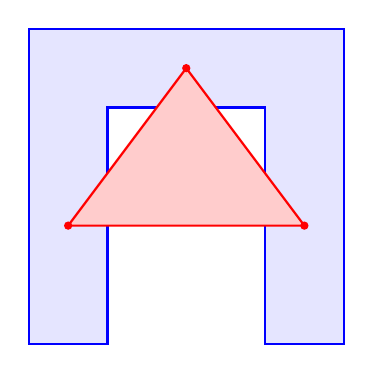
\begin{tikzpicture}[scale=0.5]
    \fill[blue!10] (0,8)--(0,0)--(2,0)--(2,6)--(6,6)--(6,0)--(8,0)--(8,8)--cycle;
    \draw[blue,thick] (0,8)--(0,0)--(2,0)--(2,6)--(6,6)--(6,0)--(8,0)--(8,8)--cycle;
    \draw[blue,thick] (2,0)--(2,6) (6,0)--(6,6);
    
    \fill[red!20] (1,3)--(7,3)--(4,7)--cycle;
    \draw[red,thick] (1,3)--(7,3)--(4,7)--cycle;
    
    \fill[red] (1,3) circle (3pt);
    \fill[red] (7,3) circle (3pt);
    \fill[red] (4,7) circle (3pt);
\end{tikzpicture}
\end{figure}
Un jugador sobrevive si no es conquistado por ningún otro. La
respuesta es el número de jugadores no conquistados.
\subsubsection*{Código}
Ver \href{https://codeforces.com/group/DH4HPwQlLU/contest/689800/submission/377242520}{código}.
